\documentclass{report}
\usepackage{graphicx}
\usepackage{verbatim}
\usepackage{pgfplots}
\usepackage[europeanresistors]{circuitikz}
\usepackage{amsmath}
\graphicspath{{./image/}}
\title{P01 report}
\author{Muhammed Juneer}
\date{march 2019}
\begin{document}
\maketitle
\chapter{Theoretical part}
\begin{center}
\begin{figure}
\centering
\begin{circuitikz}\draw
(0,0) to[battery] (0,4)
  to[resistor] (4,4) -- (4,0)
  to[resistor] (0,0)
;
\end{circuitikz}

\caption{Electrical circuit diagram}
\end{figure}
\end{center}
\section{Circuit calculation}
Theoretical calculation of the circuit
V1=1.7V
$R1=2\Omega$
R2=8ohm\\
$VR =(R\times VT)/RT$\\
$VR1= (R1 \times V1) / RT$ =  V\\
$VR2= (R2 \times V2)/ RT$ =  V\\



\begin{figure}[hbt!]
\begin{center}
\begin{tabular}{ |c|c| } 
\hline
V1 & V \\ 
R1 & ohm \\ 
R2 & ohm \\
UR1 & V \\ 
UR2 & V \\
\hline
\end{tabular}
\end{center}
\end{figure}
\begin{center}
\begin{tikzpicture}
\begin{axis}[axis lines = left,
xlabel = $R2$,
ylabel = $U(R2)$,
xmin=0,
xmax=10]
\addplot [black, very thick]{12.5*x(x+3)};
\end{axis}
\end{tikzpicture}
\end{center}

\chapter{Practical part}
Practical Calculation
\section{‘Work with GEDA programs'}
\subsection{'Work with gschem'}
\begin{figure}[hbt!]
\centering
\caption{Circuit Diagram createed in gscehm}
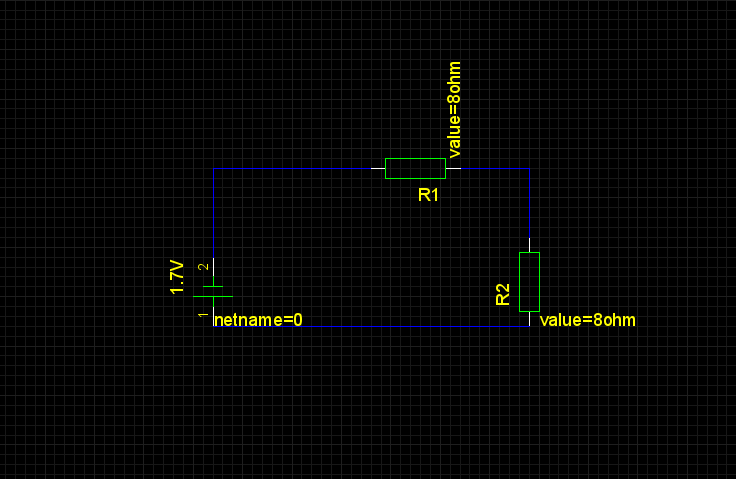
\includegraphics[width=\textwidth]{01.png}
\end{figure}
\subsection{'Work with gnetlist'}

\begin{figure}[hbt!]
\centering
\caption{The plotted graph after using ngspice}
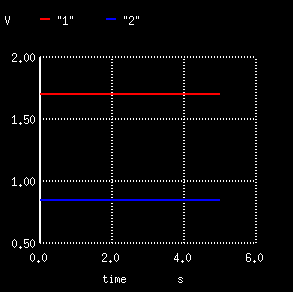
\includegraphics[width=\textwidth]{02.png}
\end{figure}


\end{document}




\end{document}